\documentclass[a4paper,12pt]{scrartcl}
\usepackage[ngerman]{babel}
\usepackage[utf8]{inputenc}
\usepackage[T1]{fontenc}
\usepackage{lmodern}
\usepackage{amsmath}
\usepackage{amssymb}
\usepackage{makeidx}
\makeindex{}
\usepackage{hyperref}
\usepackage{csquotes}
\usepackage{graphicx}

\usepackage[backend=biber,style=numeric]{biblatex}
\addbibresource{bibliography.bib}


%\renewcommand{\thesection}{Sitzung \Roman{section}: }
%\usepackage{titlesec}
%\titlelabel{Sitzung \thesection{} --- }
\title{Human Factors in Security and Privacy}
\author{\href{mailto:magnus.berendes@fau.de}{magnus.berendes@fau.de}}
\date{\today}
\begin{document}
\maketitle

\vfill
\begin{centering}
	Corrections, annotations and pull requests appreciated
	\\
\end{centering}


\newpage

\tableofcontents
\newpage
\printindex
\printbibliography
\newpage

\section{Introduction}
\begin{itemize}
	\item
		What is security?\index{Security}
		\begin{itemize}
			\item
				Protect the right thing in a right way (Anderson)
			\item
				Risk management: Trade-off between risk of attack and cost of protection
		\end{itemize}
	\item
		Defining Security:
		\begin{itemize}
			\item
				Goals: \textit{what} to protect

				Security properties of assets: CIA\index{CIA} (Confidentiality, Integrity, Availability)
			\item
				Threats: \textit{against what/whom} to protect
			\item
				Means: \textit{how} to protect

				Safeguards (attack prevention) and Countermeasures (detection and response)
		\end{itemize}
	\item
		Human Factors as Protection Means:
		\begin{itemize}
			\item
				Security management processes: policies, rules, decisions
			\item
				Usable security
			\item
				User education and training (apply with care!)
		\end{itemize}

	\item
		Security-questions to ask:
		\begin{itemize}
			\item
				System:
				\begin{itemize}
					\item
						Technical structure/organization
					\item
						Stakeholders: user types, service providers
					\item
						Assets: what should be protected?
				\end{itemize}
			\item
				Security goals? CIA?
			\item
				Threats/Attackers?
				\begin{itemize}
					\item
						Which threats are possible, probable, incur high losses?
					\item
						Incentives of the attackers?
					\item
						Resources/capabilities of the attackers?
				\end{itemize}
			\item
				Does the security measure protect against these attacks?
			\item
				If yes, is the protection \textit{effective}?
				\begin{itemize}
					\item
						Cost of protection vs. attack risk
					\item
						Are users capable of the required behavior?
				\end{itemize}
			\item
				Is it \textit{efficient}?
				\begin{itemize}
					\item
						Cost of protection (money, time, user effort (!) ) vs. attack risk
				\end{itemize}
		\end{itemize}
	\item

		\begin{figure}[ht]
			\centering
			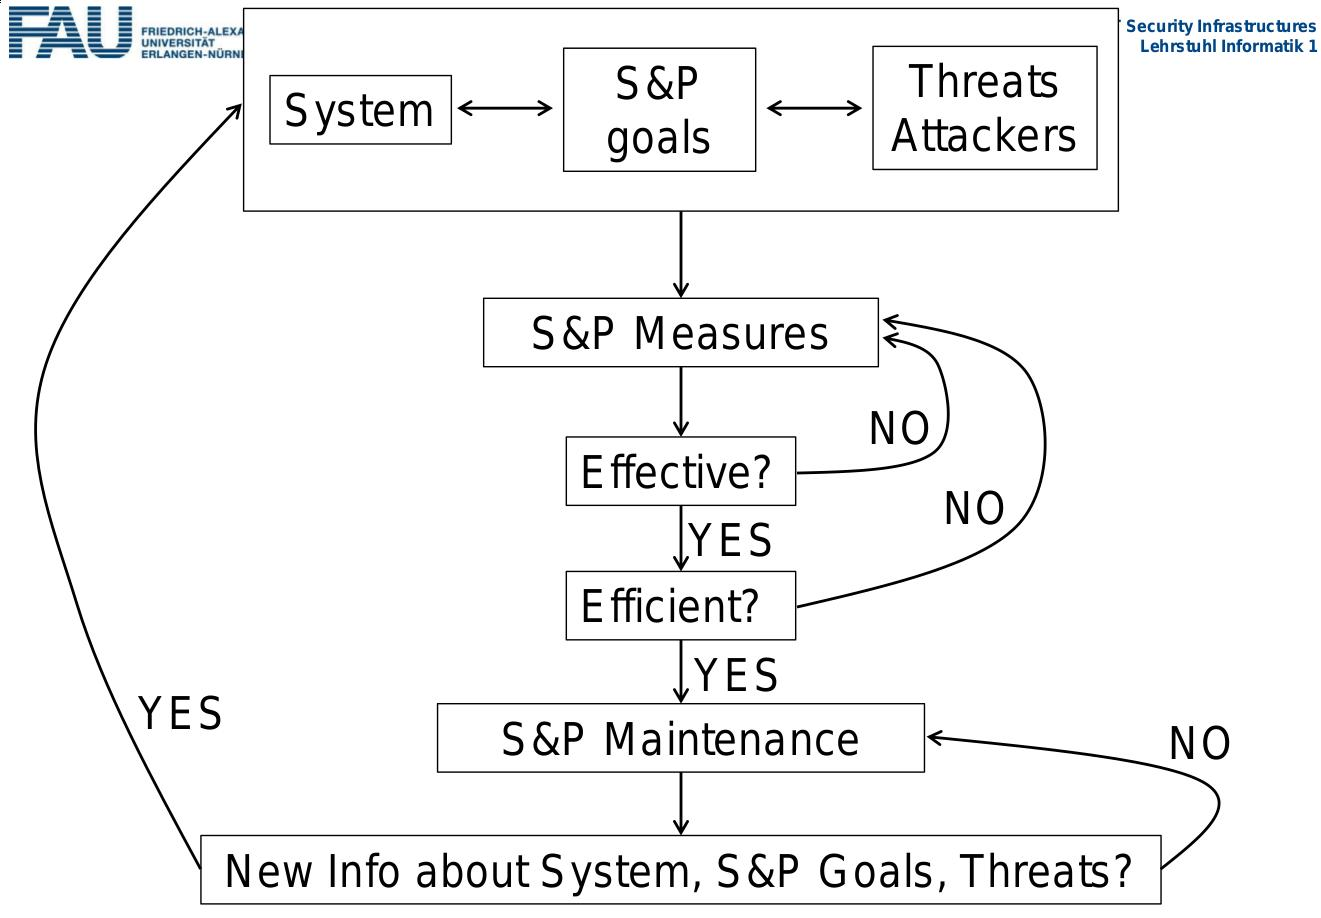
\includegraphics[
			width=0.8\textwidth]{security_process.jpg}
		\end{figure}

	\item
		Many S\&P measures offer bad trade-offs to the user: not much (subjective) gain of security, but a hassle
	\item
		\textit{Authorization}: \index{Authorization}
		\begin{itemize}
			\item
				Identification (e.g. login name)
			\item
				Plus authentication (e.g. password)
		\end{itemize}
\end{itemize}



\section{Passwords}
\begin{itemize}
	\item
		Security goals:
		\begin{itemize}
			\item
				Keep the bad guys out
			\item
				Don't lock me out!
		\end{itemize}
	\item
		Traditional password advice: strong (hard to guess), don't use it anywhere else, don't write it down, don't share it, change it often
	\item
		Do people follow this advice? No!
\end{itemize}
\subsection{Users are not the enemy}
\begin{itemize}
	\item
		\fullcite{usersenemy}
	\item
		Asked users about their password construction, frequency of use of different passwords, password recall
	\item
		Password diaries: write down all \enquote{happenings} around the password based authentication
	\item
		Findings:
		\begin{itemize}
			\item
				Users do not comply with policies
			\item
				but are not being wicked or stupid:
			\item
				They lack the right mental models of threats
			\item
				Password mechanisms lack user-centered design: not aligned with human memory capacities, not aligned with workflows (working together, delegating)
		\end{itemize}

		$\Rightarrow$ People chose weak passwords, reuse passwords, write them down, share them
	\item
		Mental Model \index{Mental Model}:
		\begin{itemize}
			\item
				Internal symbolic representation of external reality
			\item
				E.g. password=key model (how do i know if the website I'm logging into is real or fake? The key fits!)
			\item
				\enquote{Hackers cannot know the name of my cat, therefore that's a safe password}
		\end{itemize}
\end{itemize}

\subsection{A large-scale study of web password habits}
\begin{itemize}
	\item
		\fullcite{florenciolarge}
	\item
		544960 web clients, 3 months
	\item
		Windows Live Toolbar component with opt-in
	\item
		Report findings: websites, password compostion statistics (passwords were not transmitted), reuse, number of login attempts, time since last login
	\item
		Numnber of accounts per user: 25
	\item
		Each password shared across 4 different sites (avg)
	\item
		Passwords used per day: 8
	\item
		Mostly only lowercase letters \textit{unless forced to do otherwise}
\end{itemize}

\subsection{Passwords \& Human capabilities}
\begin{itemize}
	\item
		Why password logins fail:
		\begin{itemize}
			\item
				Failure to recall pssword

				Limited capacity of memory, decay over time, only unaided recall (no cues), items are non-meaningful, passwords are confused (items are similar and compete in memory), remember old password
			\item
				Typing errors

				no feedback on failure, needs to be 100\% correct
			\item
				Incorrect User ID
			\item
				User ID $\leftrightarrow$ password confusion
			\item
				Lock out after 3 attemps:

				Increasing to 10 tries decreases resets by 45\%
		\end{itemize}
	\item
		\fullcite{inglesanttrue}
		\begin{itemize}
			\item
				Data collection:  password diaries and interviews at two companies
			\item
				Conclusion very similar to \enquote{Users are not the enemy} from 1999 --- no positive changes after 10 years
		\end{itemize}
	\item
		\fullcite{florenciosecurity}
		\begin{itemize}
			\item
				Policies concentrate on forcing users to produce \enquote{strong} passwords
			\item
				Analysed \index{Minimal strength of password policies} minimal strength of password policies over 75 websites
			\item
				Minimal strength of a password policy: $N_{min} \log_2 C$

				$N_{min}$: minimal length, $C$: Character Space
			\item
				Analyses strength of the policy, not the password (strength of \enquote{password} is roughly the same as of \enquote{p4\$\$w0rd}, policy of the latter is much stronger)
		\end{itemize}
	\item
		Strength of password policies in the wild: FAU IdM much stronger than the rest ($48 > 20-27$)

		Sites with advertising often much weaker policies $\Rightarrow$ want user to sign up, password policies prevent that!
\end{itemize}
\subsection{Attacks on passwords}
\begin{itemize}
	\item
		Client: local attacks (shoulder surfing, post-its), social engineering, keyloggers
	\item
		Network:
		eavesdropping, MitM
	\item
		Server frontend: Online guessing (brute-force/dictionary) --- breadth-first (target all accounts), depth-first (target particular account), stealthy attacks (distributed in time)
	\item
		Server backend: offline guessing (prerequisite: obtain password database)
	\item[$\Rightarrow$] strong password policies protect against offline guessing attacks --- offline guessing attacks only feasible when password database is leaked, leak is not detected and passwords are salted and hashed
	\item
		Lookup tables/Rainbow tables: TODO
		\begin{itemize}
			\item
				Pre-compute hashes of passwords and look them up
			\item
				Password spaces quite big (10 ULNS policy needs more than $2^{65}$ hashes $ \mathrel{\widehat{=}} 1000$ Exabyte)
		\end{itemize}
	\item
		Online-offline chasm:
		\begin{itemize}
			\item
				Strength of passwords against online guessing: $10^4 - 10^6$ guesses
			\item
				Strength of passwords against offline guessing: $10^{14} - 10^{20}$ guesses
		\end{itemize}
		
	\item
		Summary to strong passwords:

		Strong passwords\dots
		\begin{itemize}
			\item
				reduce risk of offline guessing (iff database is hashed and salted)
			\item
				reduce risk of online guessing (but with lock-out and monitoring much weaker passwords are sufficient)
			\item
				might reduce risk against shoulder surfing and insider guessing
			\item
				don't protect against: malware, phishing, network attacks
			\item
				might increase risk of password reuse and writing down
		\end{itemize}
\end{itemize}

\subsection{Password Reuse}
\begin{itemize}
	\item
		\fullcite{tangledpasswordreuse}
		\begin{itemize}
			\item
				Study of password reuse with leaked passwords from eleven web sites
			\item
				Lots of reuses: 43\% identical, 19\% substrings
			\item
				Often tricks to transform passwords to comply with policies
		\end{itemize}
	\item
		\fullcite{florencio2014password}
		\begin{itemize}
			\item
				Lots of effort to remember which password belongs to which account \\
				($\log_2(N!)$, for N unique and random passwords)
			\item
				Unique passwords is not the optimal solution $\Rightarrow$ optimally, people should reuse passwords, group by account value and probability of compromise
		\end{itemize}
	\item
		Password Sharing
		\begin{itemize}
			\item
				Reasons for password sharing: practical needs (if something happens to me, delegation, disabilities), social norms (as a sign of trust, to show you're not paranoid, I'm a normal, nice, helpful person)
		\end{itemize}
	\item
		Password Change
		\begin{itemize}
			\item
				\fullcite{zhang2010security}
			\item
				Access to expired passwords at university, assuming knowledge of at least one password, guessed 17\% in 5 tries or lower (online), 41\% in under 3 seconds of offline attacking
		\end{itemize}
	\item
		Password Management 101
		\begin{itemize}
			\item
				Providers:
				\begin{itemize}
					\item
						Reasonable password policies and SSO
					\item
						Protection from offline guessing (hashed and salted, detect offline attacks e.g. with decoy accounts)
					\item
						Protection from online guessing (lock out after some failures, detect stealth attacks)
					\item
						Be prepared (usable and secure account recovery mechanisms, actionable strategies for the case of mass breaches)
				\end{itemize}
			\item
				Users
				\begin{itemize}
					\item
						Group passwords by account importance and attack probability (non important passwords can be reused; are users capable of distinguishing non/important accounts? Of determining attack probability?)
					\item  
						Don't reuse passwords on really important accounts
					\item
						Use aids for password management (password managers, secure writing down)
				\end{itemize}
		\end{itemize}
	\item
		Alternatives to passwords: graphical authentication, biometrics, tokens, 2FA
\end{itemize}

\section{Usable Security}
\begin{itemize}
	\item
		Usability: the extent to which a product can be used by specified users to achieve specified goals with effectiveness, efficiency and satisfaction in a specified context of use.
		\begin{itemize}
			\item
				Effectifeness: accuracy and completeness
			\item
				Efficiency: resources expended in relation to accuracy and completeness
			\item
				Satisafction: freedom from discomfort, and positive attitude to use of product
			\item
				context of use: characteristics of the users, tasks and environment
			\item
				Goal: intended outcome
			\item
				Task: activities required to achieve a goal
		\end{itemize}
	\item
		Usability Intervention at IBM 1989
		\begin{itemize}
			\item
				Field study: user group, environment, task (not authenticate, but \textit{do these 4 transactions})
			\item
				3 iterations (from mock-up to test code)
			\item
				100\% return on invested money, through time  saved while authenticating
		\end{itemize}
	\item
		\fullcite{johnnyencrypt}
		\begin{itemize}
			\item
				Security software is usable if people who are expected to use it:
				\begin{enumerate}
					\item
						Are reliably made aware of the security tasks they need to perform
					\item
						are able to figure out how to successfully perform those tasks
					\item
						don't make dangerous errors
					\item
						are sufficiently comfortable with the interface to continue using it
				\end{enumerate}
			\item
				experienced email users, no knowledge in cryptography in a lab, 12 participants
		\end{itemize}
	\item
		\fullcite{johnny2015}
		\begin{itemize}
			\item
				10 pairs of students, exchange tax return information with Mailvelope
			\item
				Results desastrous, only 1 pair completed the task (one of them knew about public key crypto before)
			\item
				All without attacker interference!
		\end{itemize}
	\item
		\fullcite{johnny2}
		\begin{itemize}
			\item
				Send sensitive data with Outlook and S/MIME, certificates are pre-loaded into mail clients of participants
			\item
				Participants don't know they are going to be attacked
			\item
				New Key attack: \enquote{computer problems}, send schedule to new address, new address has unmatching key from old address
			\item
				New Identity attack: \enquote{working from home}, new hotmail email with a new public key and misspelled email address (sara instead of sarah)
			\item
				Unsigned message attack: attacker impersonates manager being annoyed, known address, unsigned mail. Send schedule to team members NOW as they really need it
			\item
				3 groups: unmodified outlook, outlook with color coding (for secure and unsecure messages) and color coding + briefing about meaning of colors
			\item
				Conclusion: usable email clients help \textit{sometimes}: resisting attacks better with color/color+briefing, clicked encrypt is worse than with unmodified

				Some users did not trust \textit{hotmail}, ability to encrypt a message for the sender taken for indicator that the sender is genuine
		\end{itemize}
	\item
		Why is usable security hard?

		Usability: the extent to which a product can be used by specified users to achieve specified goals with effectiveness, efficiency and satisafaction in a specified context of use
		\begin{itemize}
			\item
				Product: Security is often integrated/part of product
			\item
				User Goals: Security = secondary goal
			\item
				Effectiveness: how can security be noticed? Often invisible
			\item
				Efficiency: additional time \& user effort
			\item
				Satisfaction: can people be satisfied with something that demands additional effort? Maybe better: low dissatisfaction?
			\item
				context of use: How to take attacks into account?
		\end{itemize}
	\item
		Benenson defintion of usable security:
		\begin{itemize}
			\item
				Usability of a security mechanism or policy
			\item
				is the extent to which the machnism or policy can be used by
			\item
				specified users
			\item
				to achieve the specified security goal (some of these goals being invisible or secondary goals to the users)
			\item
				and the specified primary goals
			\item
				with effectiveness, efficiency and satisfaction (or at least with low dissatisfaction)
			\item
				during the execution of the specified primary user tasks
			\item
				in a specified context of use
			\item
				including the specified attacks
		\end{itemize}
\end{itemize}
\subsection{Beyond Usability}
\begin{itemize}
	\item
		Is usability \& security a trade-off? long random passwords, single password per account, encrypted email, \dots
		\begin{itemize}
			\item
				Security versus Usability: security restricts/prohibits, usability enables
			\item
				Security aligned with Usability: Usability enables actions with desirable results, security restricts actions with undesirable results
		\end{itemize}
	\item
		Can't just add security to finished product $\Rightarrow$ usability will suffer
	\item
		Approaches to usable security (Apply in this order!)
		\begin{itemize}
			\item
				Invisible security: Make it just work, automated and invisible
			\item
				Understandable security: Make it visible and intuitive
			\item
				Train the users: effort should match benefit
		\end{itemize}
	\item
		Alternatives to passwords for web authentication:
		\begin{itemize}
			\item
				Criteria: Usability; Security/Privacy; Deployability
			\item
				Evaluated 35 alternative techniques: graphical passwords/PINs, Biometrics, Tokens, 2FA
			\item
				Results: many techniques would be better for security and privacy buuuut none has better deployability (for Web)
		\end{itemize}
	\item
		Usability criteria for web authentication:
		\begin{itemize}
			\item
				Memorywise (quasi) effortless
			\item
				Scalable for users (many accounts)
			\item
				Nothing to carry (or something the user carries anyway)
			\item
				Physically effortless (beyond pressing a button)
			\item
				Easy to learn
			\item
				Efficient to use (time)
			\item
				Infrequent errors
			\item
				Easy recovery from loss
		\end{itemize}

		Security and privacy criteria: resilience to
		\begin{enumerate}
			\item
				Physical observation
			\item
				targeted impersonation (having personal info about user does not help)
			\item
				throttled guessing (guessing attempts are constrained by service provider)
			\item
				Unthrottled guessing (attacker constrained only by computational resources)
			\item
				Internal observation (intercept users input)
			\item
				Leaks at other service providers
			\item
				Phishing
			\item
				theft of physical token (or at least pin protection)
			\item
				No trusted third party
			\item
				Explicit consent (authentication cannot be startet without user knowledge or consent)
			\item
				Unlinkable (colluding service providers cannot track the users from their authentication data)
			\item
				Privacy-protecting (does not reveal additional information about the user to the service provider / attacker
		\end{enumerate}

		Deployability Criteria
		\begin{enumerate}
			\item
				Accessible
			\item
				Low cost per user
			\item
				Server-compatible
			\item
				Browser-compatible
			\item
				Mature (User testing, open source implementations, real-world deployments)
			\item
				Non-proprietary
		\end{enumerate}
	\item
		Why doesn't Jane protect her Privacy? Renaud et.al.
		\begin{itemize}
			\item
				Qualitative study
		\end{itemize}
\end{itemize}

%\section{Example exam questions}
\subsection{Passwords}
\begin{itemize}
	\item
		Factual questions
		\begin{itemize}
			\item
				How would you define a \enquote{strong} password?


			\item
				Discuss in which cases requiring passwords of pre-defined \enquote{strength} makes sense, and in which cases it does not make sense
			\item
				What are security and usability problems of password usage? How can they be mitigated? (at least, partially)
			\item
				Which factors should be taken into account when an organization defines a password policy?
		\end{itemize}
	\item
		Transfer questions
		\begin{itemize}
			\item
				What is a secure and usable password?
			\item
				What be your personal advice on the handling of passwords to a home computer user? What are advantages and disadvantages of your advice?
			\item
				What does it mean for an authentication mechanism to be usable? To be secure?
			\item
				Which alternative authentication mechanisms do you know? How do they compare to passwords in terms of security and usability?
			\item
				How would you nvestigate security and usability of an authentication mechanism?
		\end{itemize}
\end{itemize}

\subsection{Usable Security}
\begin{itemize}
	\item
		How would you define usability?

		Inwiefern ein Produkt genutzt werden kann, um ein bestimmtes Ziel zu erreichen, im Hinblick auf Effektivität, Effizienz und Zufriedenheit in einem genau spezifizierten Kontext
	\item
		How should usability definition be adapted when reasoning about usability of security?

		Erstes Johnny paper

		Security software ist usable, wenn die Personen, die die Software benutzen sollen:
		\begin{enumerate}
			\item
				zuverlässig auf Security tasks aufmerksam gemacht werden
			\item
				herausfinden können, wie sie diese Tasks erfolgreich bewältigen können
			\item
				keine gefährlichen Fehler machen (können)
			\item
				mit dem Interface zufrieden genug sind, um es weiter zu benutzen
		\end{enumerate}
	\item
		What does it mean for a security mechanism or policy to be usable?

		Ein mechanismus oder eine Policy ist usable

		\begin{itemize}
			\item
				The extent to which the mechanism or policy can be used by
			\item
				Specified users
			\item
				Um ein bestimmtes security goal (manche davon unsichtbar oder secondary für den user)
			\item
				und das primary goal zu erreichen
			\item
				Mit Effektivität, Effizienz und Zufriedenheit
			\item
				Während der Ausführung der spezifizierten primary tasks
			\item
				in einem spezifizierten context
			\item
				unter Einbezug von spezifizierten Attacken
		\end{itemize}
	\item
		What happens if a secure system has bad usability? Examples?

		user finden work-arounds, benutzen unsichere Systeme
	\item
		How can usability of security mechanisms be tested?
		
		User study with role playing
	\item
		What is the relation between security and usability? In which cases do they constitute a trade-off? How can they be aligned with each other?

		Security verbietet, usability erlaubt

	  Usability erlaubt gute Dinge, Security verbietet böse Dinge

		Im Besten Fall unsichtbare Security, funktioniert einfach!
	\item
		Which three approaches do you know making security usable? Discuss advantages and disadvantages, give examples

		Unsichtbare Security, funktioniert einfach, technische Limits durch schlechte Accuracy, manchmal auch nicht sinnvolle Sachen tun wollen

		Understandable security: sichtbar und intuitiv machen. Schwierig unbedarften Nutzern die Hintergründe näher zu bringen, passende Metaphern/Analogien zu finden

		User education: Funktioniert nicht so gut, kostet Zeit und Geld (lohnt sich oft nicht $\Rightarrow$ phishing education!), User muss Dinge verstehen,  User muss motiviert sein!
	\item
		What other system properties, apart from usability should be satisfied in order for the system to be accepted
	\item
		You are commisioned to develop a security mechanism X / security policy Y. How would you organize the development process?

		Identify S\&P Goals and attacks, measures, effective?, efficient?

		Sinnvollerweise security schon von Anfang an der Entwicklung Teil des Produktes. Oft schwierig Security später mit einzubauen
\end{itemize}

\subsection{Cyberfraud}
\begin{itemize}
	\item
		Why is phishing an important security threat? What difficulties people have in recognizing phish?

		Passwörter können abhanden kommen, schwierig automatisch zu identifizieren, kann über verschiedene Kanäle kommen.
		User haben falsche Entscheidungs strategien um festszustellen was Phishing ist: (Email für mich, von normaler Firma, die machen das so), (Neugier, Plausibler Content), schauen oft nur auf Content der Website, nicht auf Security Indicators
	\item
		How to determine which measures against phishing are economically justifiable? Which kind of data you need in order to answer the question? (no need for statistics from the lecture)

		Jährliche Kosten durch Phishing / Potentiell betroffene Personen (Internet User) = Kosten / Person / Jahr

		Kann man über Mindestlohn in Zeit umrechnen, ist nicht so viel
	\item
		Why do Nigerian scammers say they are from Nigeria?

		Jemand der so eine doofe Geschichte glaubt, kann quasi dazu gebracht werden alles zu glauben. \enquote{Intelligentere} Leute fallen da schon nicht drauf rein, sind also keine leichten Ziele
	\item
		What psychological tricks make people commit errors of judgement and fall for scam in consequence?

		An Vertrauen und Autorität appelieren, große Gewinne, künstliche Knappheit (nur jetzt, sonst zu spät!), commitment (immer nur kleine Schritte machen)
	\item
		Explain principles of psychological influence with security-related examples
		\begin{itemize}
			\item
				Erwiderung: Phishing email (wir haben das für dich getan, jetzt musst du das hier noch bestätigen\dots und dein Passwort eingeben)
			\item
				Commitment: Scam emails
			\item
				Social proof: In Phishing Email: \enquote{5000 Personen haben die neuen AGBs schon bestätigt\dots und ihr Passwort eingegeben}
			\item
				Authority: Warnungen mit Angstmachen?
			\item
				Liking: 
			\item
				Scarcity: In Scam Emails (schnell machen!)

		\end{itemize}

	\item
		(Transfer) Is user education a good measure against phishing or social engineering for home computer users / for employees? Argue your opinion!

		For home users: effort doesn't match benefit, training might be infeasible or have negative effects, erzeugt Angst (bringt Leute mehr davon ab Online Banking zu benutzen als tatsächlicher Identity Theft!)
\end{itemize}

\subsection{User education, Awareness, training}
\begin{itemize}
	\item
		Awareness, education, training: what are the differences between these terms?

		Awareness = Wissen um Angriffe, education = Wissen um Verteidignungsmaßnahmen, Training = Richtiges Verhalten
	\item
		What are pros and cons of security measures that try to change the users by means of awareness, education and training?

		Schwierig für User, zu schwierig. Gibt Verantwortung an die falschen (devs und admins sollten für Sicherheit verantworlich sein!). Macht Leuten Angst (Online banking, id theft vs. fear mongering)
	\item
		In which cases is a fear-inducing security message a good idea? (Explain the extended parallel processing model, awareness poster for identity theft)

		Stimulus kommt an (nachricht, warnung)

		First appraisal: perceived threat = entweder weiter zu 2nd appraisal oder kein Threat wahrgenommen

		Second appraisal: Perceived efficay, dann wenn Wirksame Gegenmaßnahme möglich protection motivation und adaptive changes, falls keine wirksamen Gegenmaßnahmen möglich/bekannt dann defensive motivation und maladaptive changes
	\item
		Which factors should be considered when designing a user education campaign?
\end{itemize}

\subsection{Warnings}
\begin{itemize}
	\item
		Compare and constrast passive and active warnings

		Passive: Indikatoren, sehr ineffektiv, oft gar nicht bemerkt

		Aktive: Unterbrechen User, oft auch ineffektiv, Automatische Antwort (einfach wegklicken), oft nicht verstanden
	\item
		What makes a good/bad warning or indicator? Examples?
	\item
		Which factors influence responses to warnings?
	\item
		Which issues arise when security experts want people to comply with security warnings?
	\item
		In which cases can non-compliance with a warning be a better decision than compliance?
\end{itemize}

\subsection{Privacy}
\begin{itemize}
	\item
		How would you define Privacy? What is the difference between privacy and confidentiality?
	\item
		How do the views on privacy differ between EU and USA?
	\item
		What is the Westin privacy index used for? What problems exist with the usage of this index?
	\item
		Explain the meaning of privacy paradox / privacy dichotomy
	\item
		Explain the rational choice theory in economics and how decision making  in privacy deviates from it
	\item
		Explain and give examples of
		\begin{itemize}
			\item
				Asymmetric information
			\item
				Bounded rationality
			\item
				Behavioral biases
		\end{itemize}
	\item
		Give examples on how the decisions to share or to withhold sensitive information are dependent on the context in which the request for information is made
		\begin{itemize}
			\item
				Seriousness
			\item
				Endowment effect / order effect
		\end{itemize}
	\item
		Why is privacy considered to be a human right? What are the serious consequences for individuals and society if privacy is violated?
		\begin{itemize}
			\item
				Feature creep, aggregation, exclusion
			\item
				Problems with the \enquote{I've got nothing to hide} argument
		\end{itemize}
	\item
		What are arguments for and against data retention?
	\item
		Is NSA-type surveillance a good measure against crime and terrorism? Argue why or why not, (depending on you opinion) and give examples
	\item
		What role does risk overestimation play in the societal and political debate about data retention / NSA surveillance? Explain how and why risk overestimation happens and what are the consequences of overreaction.
\end{itemize}

\end{document}
